\documentclass[tikz,border=6pt]{standalone}
\usepackage{amsmath,amsfonts}
\usetikzlibrary{positioning,shapes,arrows.meta,decorations.pathreplacing,calc}

\begin{document}
	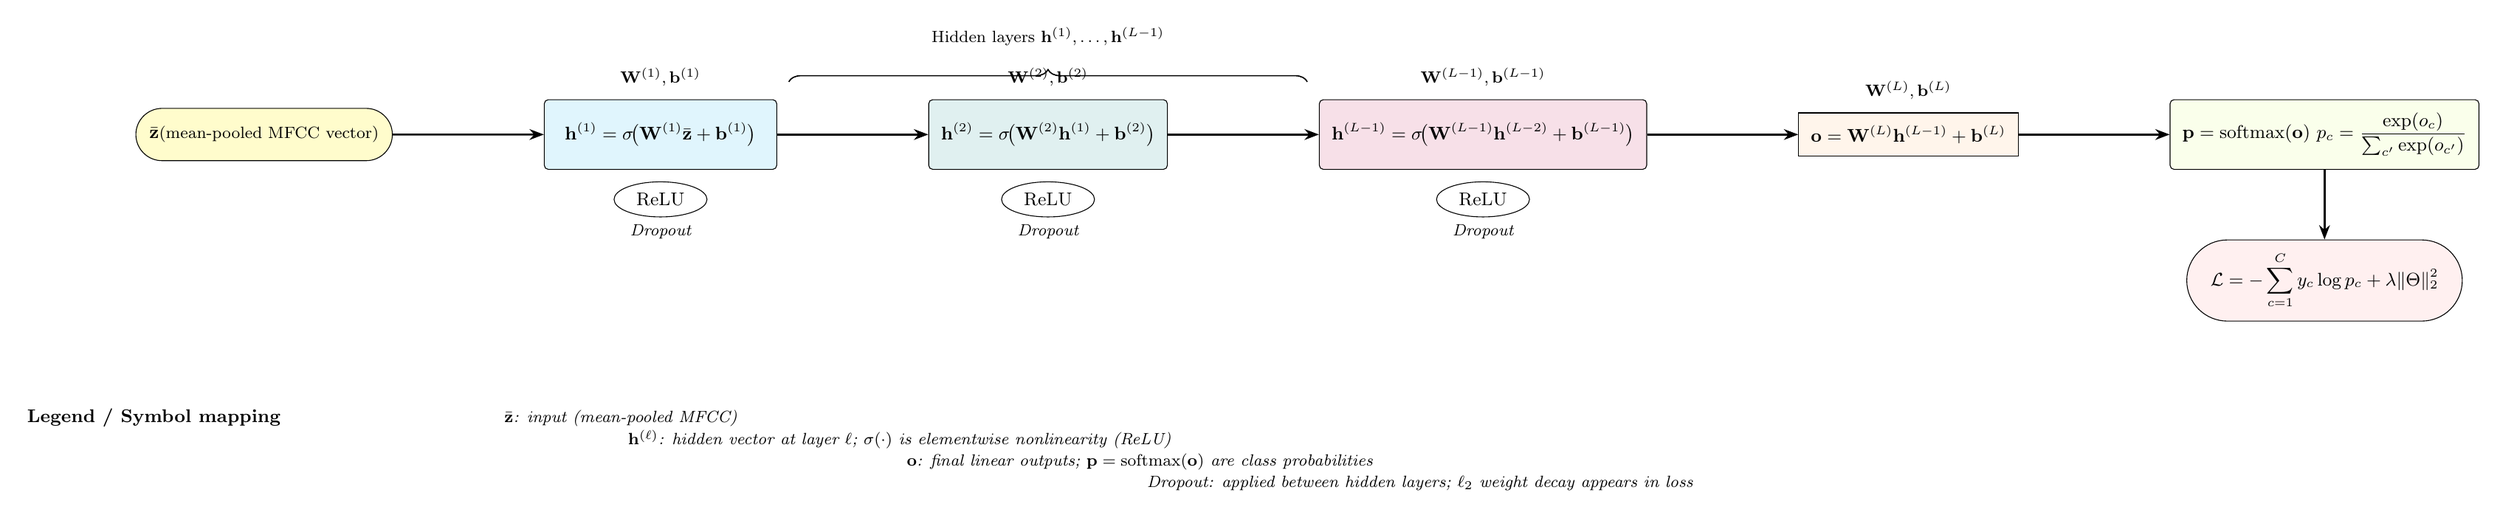
\begin{tikzpicture}[
		node distance=10mm and 18mm,
		every node/.style={font=\small},
		input/.style={draw, rounded rectangle, fill=yellow!20, inner sep=6pt, minimum width=36mm, minimum height=9mm},
		layer/.style={draw, rectangle, rounded corners=2pt, inner sep=6pt, minimum width=40mm, minimum height=12mm},
		act/.style={draw, ellipse, inner sep=3pt, minimum width=16mm, fill=white},
		op/.style={draw, rectangle, fill=green!10, inner sep=6pt, minimum width=34mm},
		arrow/.style={-Stealth, line width=0.9pt},
		note/.style={font=\footnotesize\itshape}
		]
		
		% Input
		\node[input] (z) {$\bar{\mathbf{z}}$ \\ \footnotesize (mean-pooled MFCC vector)};
		
		% Layer 1
		\node[layer, right=of z, xshift=8mm, fill=cyan!12] (L1) {
			$\mathbf{h}^{(1)}=\sigma\!\big(\mathbf{W}^{(1)}\bar{\mathbf{z}}+\mathbf{b}^{(1)}\big)$
		};
		\node[act, below=2mm of L1] (relu1) {ReLU};
		\node[note, below=0mm of relu1] (do1) {Dropout};
		
		% Layer 2
		\node[layer, right=of L1, xshift=8mm, fill=teal!12] (L2) {
			$\mathbf{h}^{(2)}=\sigma\!\big(\mathbf{W}^{(2)}\mathbf{h}^{(1)}+\mathbf{b}^{(2)}\big)$
		};
		\node[act, below=2mm of L2] (relu2) {ReLU};
		\node[note, below=0mm of relu2] (do2) {Dropout};
		
		% Middle hidden (representing ... up to L-1)
		\node[layer, right=of L2, xshift=8mm, fill=purple!12] (Lk) {
			$\mathbf{h}^{(L-1)}=\sigma\!\big(\mathbf{W}^{(L-1)}\mathbf{h}^{(L-2)}+\mathbf{b}^{(L-1)}\big)$
		};
		\node[act, below=2mm of Lk] (reluk) {ReLU};
		\node[note, below=0mm of reluk] (dok) {Dropout};
		
		% Output linear layer
		\node[op, right=of Lk, xshift=8mm, fill=orange!8] (out) {
			$\mathbf{o}=\mathbf{W}^{(L)}\mathbf{h}^{(L-1)}+\mathbf{b}^{(L)}$
		};
		
		% Softmax and probabilities
		\node[layer, right=of out, xshift=8mm, fill=lime!8] (soft) {
			$\mathbf{p}=\mathrm{softmax}(\mathbf{o})$\\[2pt] $p_c=\dfrac{\exp(o_c)}{\sum_{c'}\exp(o_{c'})}$
		};
		
		% Loss box
		\node[draw, rounded rectangle, below=12mm of soft, fill=red!6, inner sep=6pt] (loss) {
			$\displaystyle \mathcal{L}=-\sum_{c=1}^C y_c\log p_c + \lambda \lVert \Theta\rVert_2^2$
		};
		
		% Connections
		\draw[arrow] (z) -- (L1);
		\draw[arrow] (L1) -- (L2);
		\draw[arrow] (L2) -- (Lk);
		\draw[arrow] (Lk) -- (out);
		\draw[arrow] (out) -- (soft);
		\draw[arrow] (soft.south) -- ++(0,-6mm) -| (loss.north);
		
		% Parameter annotations
		\node[above=1mm of L1] {\footnotesize $\mathbf{W}^{(1)},\mathbf{b}^{(1)}$};
		\node[above=1mm of L2] {\footnotesize $\mathbf{W}^{(2)},\mathbf{b}^{(2)}$};
		\node[above=1mm of Lk] {\footnotesize $\mathbf{W}^{(L-1)},\mathbf{b}^{(L-1)}$};
		\node[above=1mm of out] {\footnotesize $\mathbf{W}^{(L)},\mathbf{b}^{(L)}$};
		
		% Legend
		\begin{scope}[shift={(0,-40mm)}]
			\node[anchor=north west] (leg) at (-42mm,-6mm) {\textbf{Legend / Symbol mapping}};
			\node[note, right=of leg, xshift=18mm, anchor=west] (s1) {
				$\bar{\mathbf{z}}$: input (mean-pooled MFCC)
			};
			\node[note, below=1mm of s1, anchor=west] (s2) {
				$\mathbf{h}^{(\ell)}$: hidden vector at layer $\ell$; $\sigma(\cdot)$ is elementwise nonlinearity (ReLU)
			};
			\node[note, below=1mm of s2, anchor=west] (s3) {
				$\mathbf{o}$: final linear outputs; $\mathbf{p}=\mathrm{softmax}(\mathbf{o})$ are class probabilities
			};
			\node[note, below=1mm of s3, anchor=west] (s4) {
				Dropout: applied between hidden layers; $\ell_2$ weight decay appears in loss
			};
		\end{scope}
		
		% Brace to show many hidden layers
		\draw[decorate,decoration={brace,amplitude=6pt},line width=0.6pt]
		($(L1.north east)+(2mm,3mm)$) -- ($(Lk.north west)+(-2mm,3mm)$) node[midway,above=5mm,font=\footnotesize] {Hidden layers $\mathbf{h}^{(1)},\dots,\mathbf{h}^{(L-1)}$};
		
	\end{tikzpicture}
\end{document}
